\begin{infocard}{\footnotesize Suma de los ángulos interiores de un triángulo}
    \begin{figure}[H]
        \centering
        \caption{La suma de los ángulos interiores de un triángulo es 180$^\circ$.}
        \label{fig:angulos_correspondientes}
        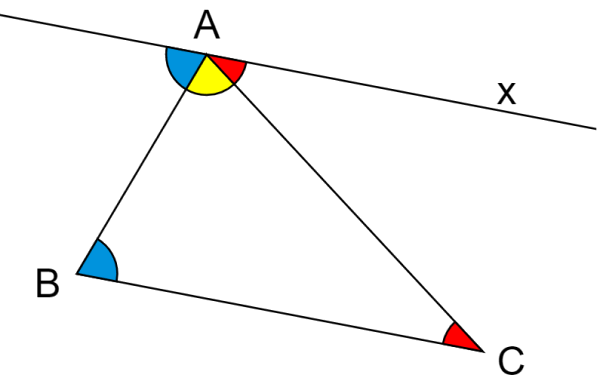
\includegraphics[width=0.8\linewidth]{../images/angulos-internos-de-un-triangulo.png}
    \end{figure}
    \[\angle {\color{colorrds}ABC}+\angle {\color{red}BCA}+\angle {\color{Goldenrod}CAB}=180^\circ\]
\end{infocard}